\section{Introduction}

\subsection{Problem Definition}

While breathing patterns offer valuable clues for detecting chronic disease, practical tools for home monitoring are missing. The existing options are simply not viable for widespread use. Hospital-grade devices are prohibitively expensive and complex, and manually reviewing audio data is an unscalable process unsuitable for real-time applications \cite{lee2025co2sensor}.

The most obvious alternative---listening to the breath---is simple and non-invasive. But it has a critical flaw. Inhales and exhales often sound remarkably alike, a similarity that confounds simple algorithms (Fig. \ref{fig:sample_waveform}). This problem is amplified by real-world conditions like background noise or differences between individuals, causing conventional acoustic methods to fail. A more sophisticated interpretive model is therefore necessary to reliably classify respiratory phases from sound alone \cite{lee2023wheezing}.

\begin{figure}[h!]
    \centering
    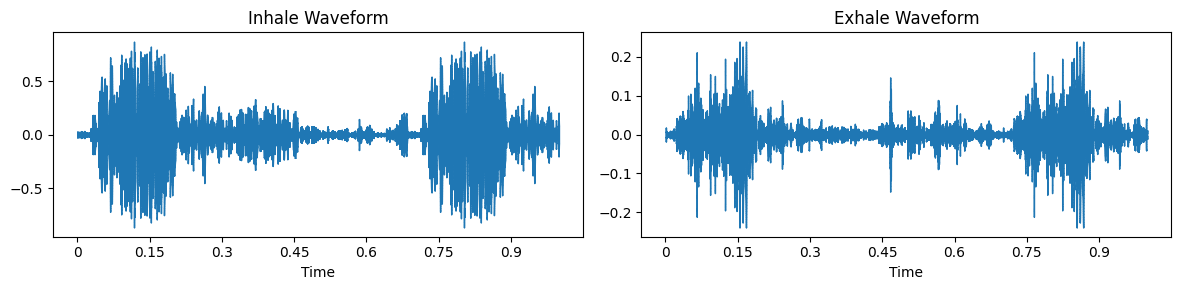
\includegraphics[width=\columnwidth]{figures/sample_waveform}	
    \caption{Example waveforms showing inhale vs exhale patterns}
    \label{fig:sample_waveform}
\end{figure}

\subsection{Research Objectives}

This study confronts the problem by designing a deep learning model specifically trained to differentiate between the subtle acoustic signatures of inhalation and exhalation. We feed a rich tapestry of acoustic information---spanning multiple spectrogram formats, frequency-domain vectors, and signal energy characteristics---into a multi-input Convolutional Neural Network(CNN).

\subsection{Dataset Overview}

The dataset provided for this study consists of 5,000 individual audio recordings of human respiratory sounds. The data is pre-partitioned into a training set of 4,000 samples and a test set of 1,000 samples. Each sample is a one-second, mono-channel audio file in the .wav format, and labled either an inhalation or an exhalation for the training set.
